\documentclass{article}

\usepackage{caption}

\usepackage{multirow}

\usepackage{graphicx}
\setlength{\abovecaptionskip}{10pt plus 3pt minus 2pt}
\setlength{\belowcaptionskip}{10pt plus 3pt minus 2pt}

\usepackage[margin=1in]{geometry}

\usepackage{hyperref}
\hypersetup{
    pdfborderstyle={/S/U/W 1},
    colorlinks=true,
    linkcolor=blue,
    filecolor=magenta,
    urlcolor=cyan,
}

\usepackage{algorithm,algpseudocode}

\usepackage{xcolor}
\usepackage{listings}
\lstdefinestyle{DOS}{
    backgroundcolor=\color{lightgray},
    basicstyle=\scriptsize\color{black}\ttfamily
}

\title{
CSE 5441 (Fall 2019, Dr. Jones)\\
\large Serial AMR (Lab 1)
}
\author{
Caleb Lehman \\
\href{mailto:lehman.346@osu.edu}{lehman.346@osu.edu}
}

\begin{document}
\maketitle

\section*{Overview}
\label{sec:overview}

For this lab, I prepared a serial \texttt{C} program to perform a serial
Adaptive Mesh Refinement (AMR)\footnote{In this case, the \emph{mesh} is static,
so the program may be more accurately described as a serial \emph{stencil
code/computation.}}. The input to the problem is a tiling of a rectuangular
grid composed of disjoint boxes along with their initial
temperatures\footnote{While the values are specifically assumed to be temperatures,
the setup is general enough to encompass any type of values. Throughout the
report, I simply refer to them as ``Domain Specific Values'' (DSV).}. The
program then iteratively updates the values in each box based on the current
values of neighboring boxes. In addition to the inputs described above, two
additional inputs are given: $\alpha$ (affect-rate), which determines the
magnitude of the effect of neighboring boxes, and $\varepsilon$ (epsilon),
which determines when convergence is reached an the program terminates.

\subsection*{Algorithm}
\label{subsec:algorithm}

Given $\alpha$, $\varepsilon$, a description of grid-aligned boxes, and initial
Domain Specific Values (DSV), the rough pseudocode for my implementation is as
follows:

\begin{algorithm}
\begin{algorithmic}[1]
\Procedure{AMR}{$\alpha$, $\varepsilon$, $N$, $Boxes$, $Initial DSV$}
\State $DSV \gets Initial DSV$
\State $DSV' \gets Initial DSV$
\While{$(\max{DSV} - \min{DSV})$ / $\max{DSV} > \varepsilon$} \label{alg:amr:convergence}
    \For{$i < N$}
        \State $DSV'[i] \gets (1 - \alpha)\cdot DSV[i] + \alpha \cdot \sum_{j\in nhbr} DSV[j]\cdot \Call{Overlap}{i, j, Boxes}$ \label{alg:amr:stencil}
    \EndFor
    \State $DSV \gets DSV'$ \label{alg:amr:commit}
\EndWhile
\EndProcedure
\end{algorithmic}
\end{algorithm}

Note the use of the $\varepsilon$ (epsilon) parameter on
line~\ref{alg:amr:convergence} to check for convergence and the use of the
$\alpha$ (affect-rate) parameter on line~\ref{alg:amr:stencil} to weight the
effect of neighboring boxes\footnote{Some boxes touch the edge of the grid, in
which case they are assigned themselves as an additional neighbor. This is
equivalent to assuming that the area outside the grid has the same DSV as the
nearest box.}.  Updated DSV are commited on line~\ref{alg:amr:commit}. The
particular implementation details can be found in the \texttt{common.c} and
\texttt{amr.c} files, which contain the code for pre-processing the input and
running the stencil code.

\subsection*{Summary}
\label{subsec:summary}

\begin{itemize}

    \item Runtimes increased when either parameter was decrease, as expected.

    \item Selected parameters $\alpha=0.1$, $\varepsilon=0.2$, which yielded a
    runtime of roughly 4 minutes to run with the
    \texttt{testgrid\textunderscore 400\textunderscore 12206} file. Full timing
    results with these parameters are presented in the
    \hyperref[sec:results]{results section}.

\end{itemize}

\newpage
\section*{Tests}
\label{sec:tests}

\subsection*{Environment}
\label{subsec:environment}

The program was developed and tested on a single node of the
\href{https://www.osc.edu/resources/technical_support/supercomputers/pitzer}{Pitzer
cluster} at the \href{https://www.osc.edu/}{Ohio Supercomputer Center}.

For development, I loaded the \texttt{intel/18.0.3} module, which allowed the
program to be compiled with version 18.0.3 of the \texttt{icc} C-compiler.

For testing, I loaded the \texttt{python/3.6-conda5.2} module, which loads a
python environment with the \texttt{NumPy}, \texttt{SciPy}, and
\texttt{Matplotlib} packages, amoung others.

\subsection*{Timing}
\label{subsec:timing}

The program was timed using several methods\footnote{Each method reports in
different units/structues, all of which were converted seconds.}:

\begin{itemize}
    \item The \texttt{time} function declared in the \texttt{time.h} header
    \item The \texttt{clock} function declared in the \texttt{time.h} header
    \item The \texttt{clock\textunderscore gettime} function declared in the \texttt{time.h} header
    \item The \texttt{UNIX} utility \texttt{time}
\end{itemize}

\subsection*{Test Files}
\label{subsec:test_files}

Dr. Jones provided several files for testing purposes:

\begin{itemize}
    \item \texttt{testgrid\textunderscore 50\textunderscore 78}: 50x50 grid with 78 boxes
    \item \texttt{testgrid\textunderscore 50\textunderscore 201}: 50x50 grid with 201 boxes
    \item \texttt{testgrid\textunderscore 200\textunderscore 1166}: 200x200 grid with 1166 boxes
    \item \texttt{testgrid\textunderscore 400\textunderscore 1636}: 400x400 grid with 1636 boxes
    \item \texttt{testgrid\textunderscore 400\textunderscore 12206}: 400x400 grid with 12206 boxes
\end{itemize}

\newpage
\section*{Results}
\label{sec:results}

The first requirement of this project was to determine values for $\alpha$
(affect-rate) and $\varepsilon$ (epsilon) such that the program converged in
between 3 to 6 minutes when run on the \texttt{testgrid\textunderscore
400\textunderscore 12206} test file. I ran a sweep over both parameters,
capturing the runtimes reported by \texttt{clock\textunderscore gettime} (see
Figure~\ref{fig:param_sweep}). As expected, the runtime increases when either
of the parameters decrease.

I selected parameters $\alpha=0.1$, $\varepsilon=0.2$ and ran the program
on each of the test files. The results are tabulated in Table~\ref{tab:runtime}.
In particular, the program took roughly 4 minutes, 21 seconds to run on the
\texttt{testgrid\textunderscore 400\textunderscore 12206} file.

\begin{minipage}{\linewidth}
    \centering
    \begin{minipage}{0.4\linewidth}

            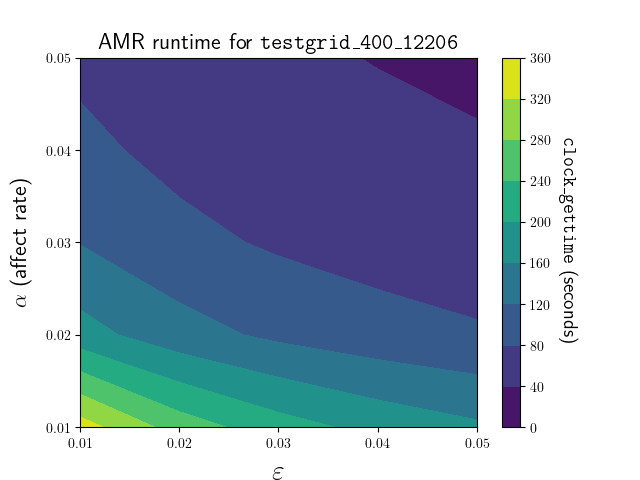
\includegraphics[width=\linewidth]{../results/testgrid_400_12206_results.png}

            \captionof{figure}{The runtime of the \texttt{amr} program on the
            \texttt{testgrid\textunderscore 400\textunderscore 12206} test file
            for various values of $\alpha$, $\varepsilon$.}
            \label{fig:param_sweep}

    \end{minipage}
    \hspace{0.02\linewidth}
    \begin{minipage}{0.45\linewidth}
        \centering
        \begin{tabular}{|l|c|c|c|c|}
            \hline
            \multicolumn{1}{|c|}{\multirow{2}{*}{Test file}} & \multicolumn{3}{|c|}{\texttt{\#include <time.h>}} & \texttt{UNIX} \\
            \cline{2-5}
            \multicolumn{1}{|c|}{} & \texttt{time} & \texttt{clock} & \texttt{gettime} & \texttt{time} \\
            \hline
            \hline
            \texttt{50,78}     & 0.00 & 0.01 & 0.02 & 0.07 \\
            \texttt{50,201}    & 0.00 & 0.07 & 0.08 & 0.12 \\
            \texttt{200,1166}  & 3.00 & 2.95 & 2.96 & 3.01 \\
            \texttt{400,1636}  & 7.00 & 7.12 & 7.13 & 7.18 \\
            \texttt{400,12206} & 261.00 & 260.47 & 261.09 & 261.18 \\
            \hline
        \end{tabular}

        \captionof{table}{Runtimes for each of the test files using
        parameters $\alpha=0.1$, $\varepsilon=0.2$. Test file names are
        abbrviated from \texttt{testgrid\textunderscore n\textunderscore m} to \texttt{n,m}.}
        \label{tab:runtime}

    \end{minipage}
\end{minipage}

\section*{Project Usage}
\label{sec:project}

This section details basic commands needed to build and run the project and is
only applicable for the code submission corresponding to this report. For full
details, see the \texttt{README} included in the code submission.

\subsection*{Building}
\label{subsec:building}

To build the \texttt{amr} executable, navigate to the top level of the
submitted directory and build as follows:

\begin{lstlisting}[style=DOS]
# Ensure that you have icc compiler

$ make
...
$ ./amr
Usage: amr [affect-rate] [epsilon]

affect-rate: float value controlling the effect of neighboring boxes
epislon    : float value determining the cutoff for convergence
\end{lstlisting}

To compile this report from source:

\begin{lstlisting}[style=DOS]
# Ensure that you have pdflatex compiler
# and that the results/ directory has
# the necessary plots for the report

$ make report
\end{lstlisting}

\subsection*{Running}
\label{subsec:running}

The syntax to run the program is:

\begin{lstlisting}[style=DOS]
$ ./amr [affect-rate] [epsilon] <[test-file]
\end{lstlisting}

\end{document}
